\providecommand{\main}{../../../..}
\documentclass[\main/dresen_thesis.tex]{subfiles}
\begin{document}
  \label{sec:looselyPackedNS:layers:pnr}
  \begin{figure}[tb]
    \centering
    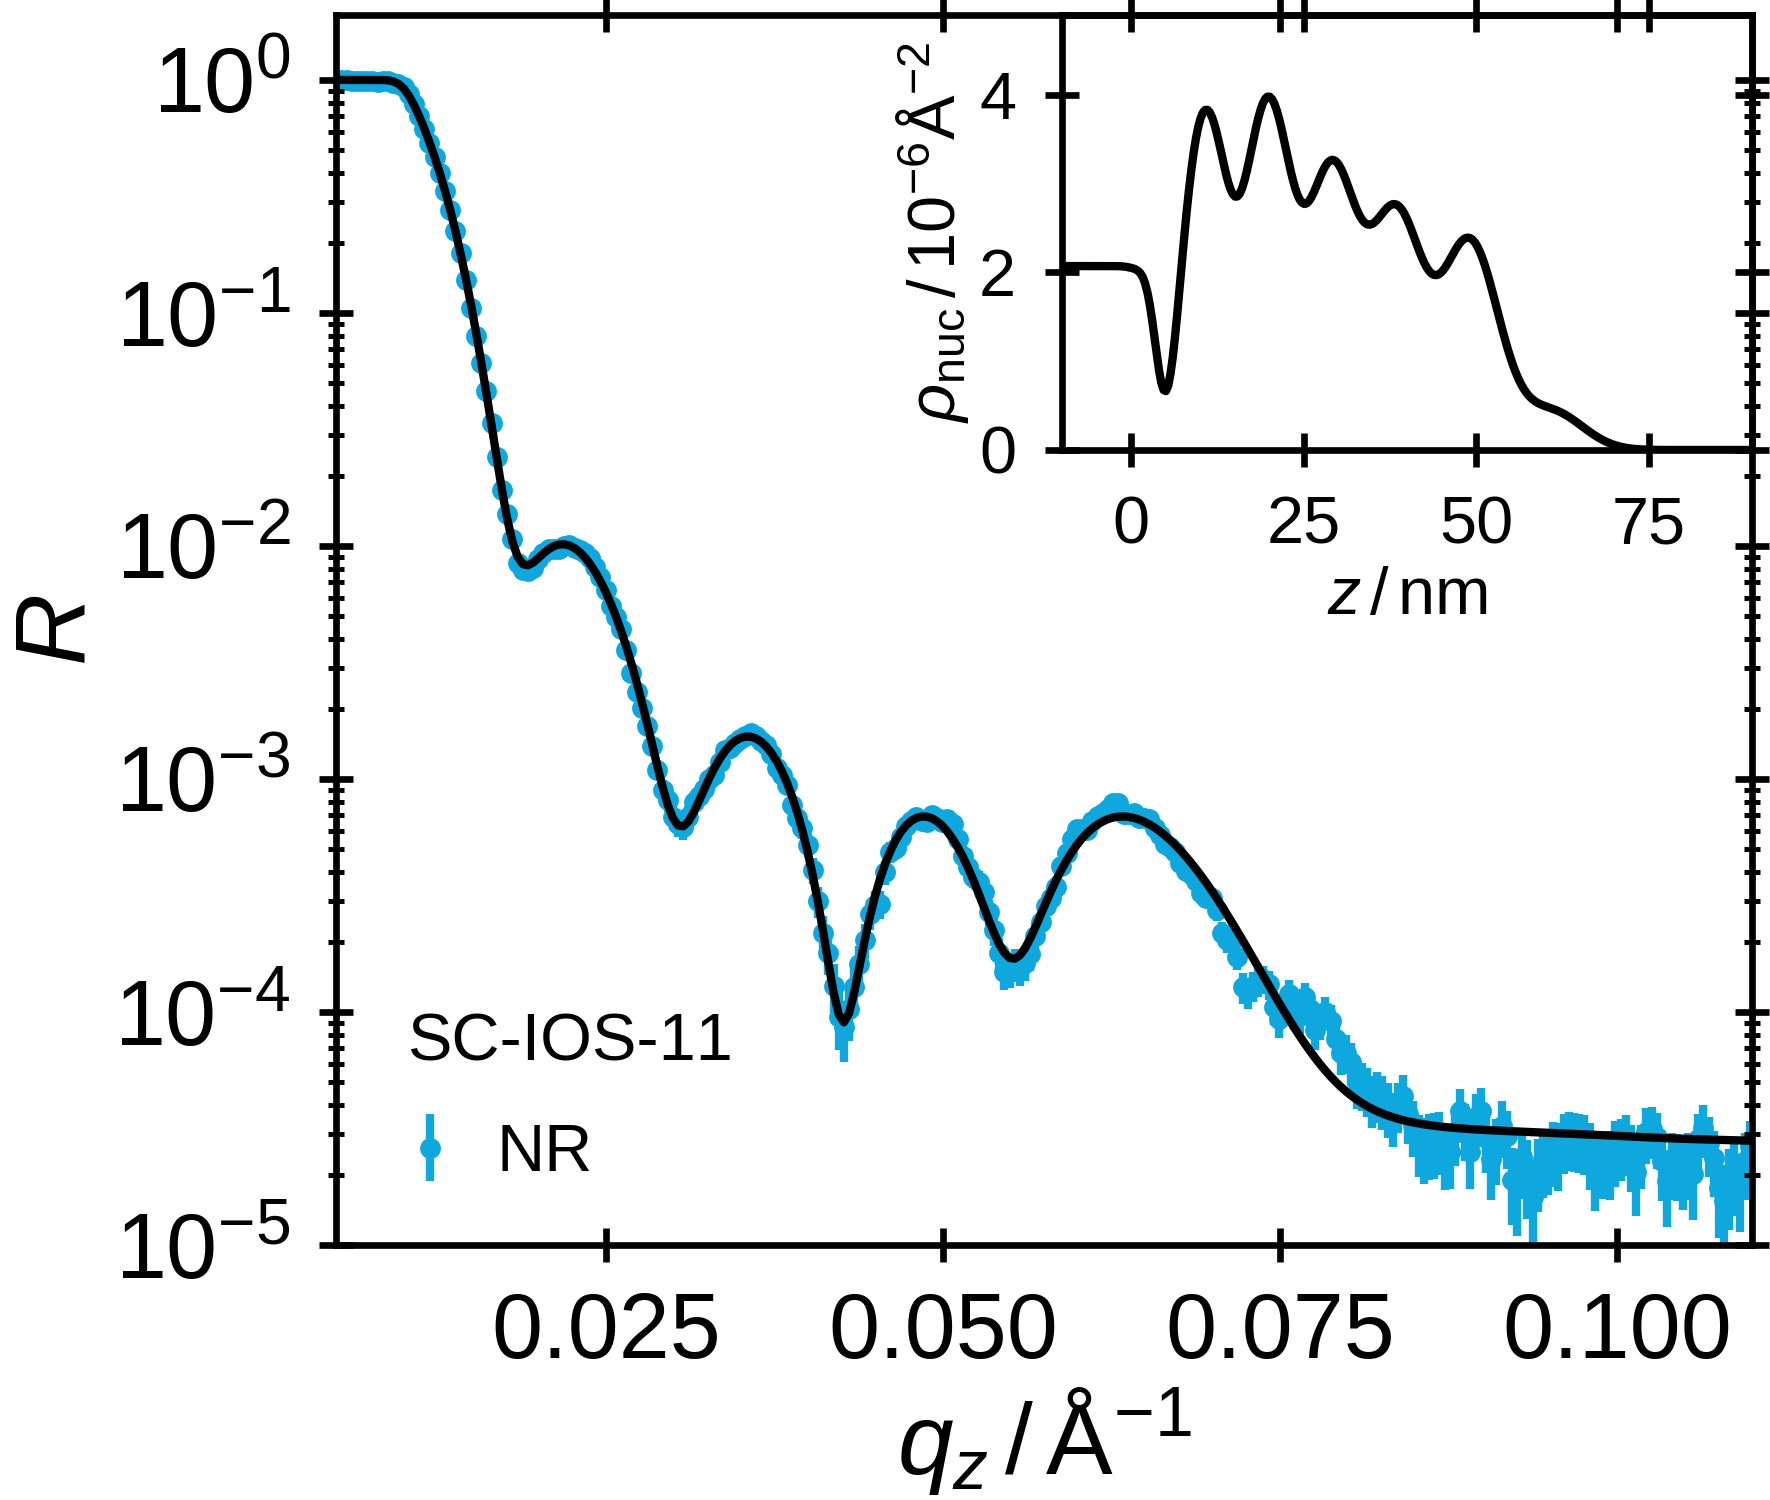
\includegraphics{looselyPackedNP_VerticalStructure_SC-IOS-11_PNR}
    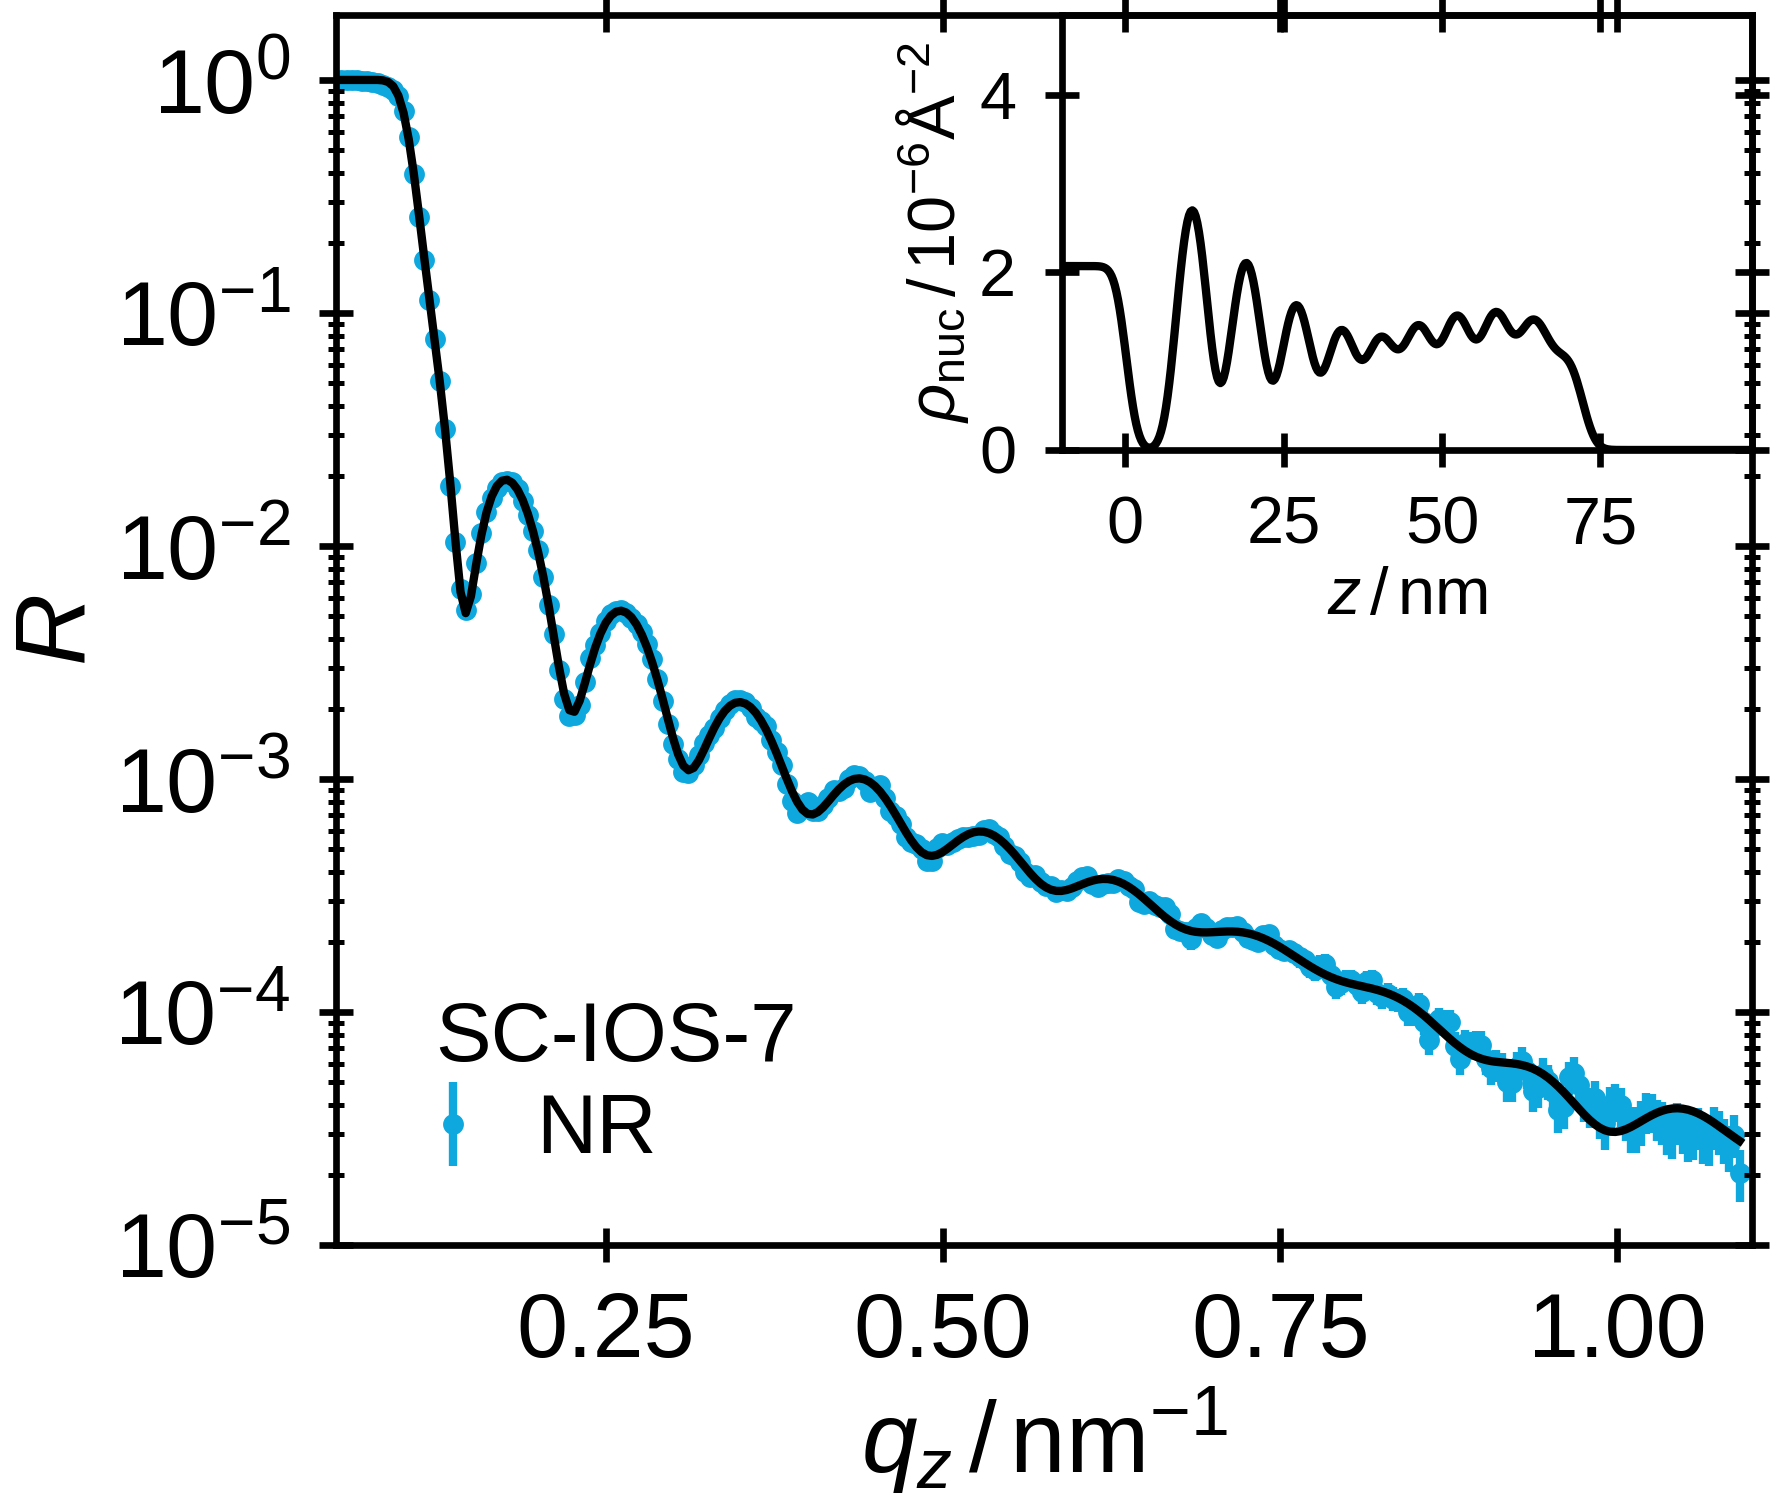
\includegraphics{looselyPackedNP_VerticalStructure_SC-IOS-7_PNR}
    \caption{\label{fig:looselyPackedNP:layer:xrr}X-ray reflectometry from SC-IOS-11 (left) and SC-IOS-7 (right). The inset shows the scattering length density model of the fitted reflectometry curve (black).}
  \end{figure}

  \begin{table}[!htbp]
    \centering
    \caption{\label{tab:looselyPackedNP:layers:pnr}Parameters for the layered nanosphere model shown in \reffig{fig:looselyPackedNP:layer:pnr}. The definitions of the parameters are analogue to \reftab{tab:looselyPackedNP:layers:xrr}.}
    \begin{tabular}{ c | l | l }
      \rule{0pt}{2ex} \textbf{NR}  & \textbf{SC-IOS-11} & \textbf{SC-IOS-7} \\
      \hline
       $\eta_1     \, / \unit{\%}$                                  & $96(1)$           & $99.2(1)$    \\
       $\eta_2     \, / \unit{\%}$                                  & $103(1)$          & $77.4(1)$    \\
       $\eta_3     \, / \unit{\%}$                                  & $89(1)$           & $59.8(1)$    \\
       $\eta_4     \, / \unit{\%}$                                  & $79(1)$           & $49.0(1)$    \\
       $\eta_5     \, / \unit{\%}$                                  & $78(1)$           & $45.4(1)$    \\
       $\eta_6     \, / \unit{\%}$                                  & $18(1)$           & $50.0(1)$    \\
       $\eta_7     \, / \unit{\%}$                                  &                   & $54.1(1)$    \\
       $\eta_8     \, / \unit{\%}$                                  &                   & $55.2(1)$    \\
       $\eta_9     \, / \unit{\%}$                                  &                   & $51.2(1)$    \\
       $\eta_{10}     \, / \unit{\%}$                               &                   & $35.4(2)$    \\
       \hline
       $\Delta z_1 \, / \unit{nm} $                                 & $-2.2(1)$        & $-0.9(1)$ \\
       $\Delta z_2 \, / \unit{nm} $                                 & $-2.8(1)$        & $-0.0(1)$ \\
       $\Delta z_3 \, / \unit{nm} $                                 & $-2.6(1)$        & $-0.6(1)$ \\
       $\Delta z_4 \, / \unit{nm} $                                 & $-2.6(1)$        & $-1.5(1)$ \\
       $\Delta z_5 \, / \unit{nm} $                                 & $-1.5(1)$        & $-2.3(1)$ \\
       $\Delta z_6 \, / \unit{nm} $                                 & $-0.2(1)$       & $-2.5(1)$ \\
       $\Delta z_7 \, / \unit{nm} $                                 &                   & $-2.4(1)$ \\
       $\Delta z_8 \, / \unit{nm} $                                 &                   & $-2.4(1)$   \\
       $\Delta z_9 \, / \unit{nm} $                                 &                   & $-2.6(1)$    \\
       $\Delta z_{10} \, / \unit{nm} $                              &                   & $-3.2(1)$   \\
       \hline
       $d_\mathrm{spacer}   \, / \unit{nm} $                        & $5.0(1)$          & $6.1(1)$  \\
       $\rho_\mathrm{spacer}\, / \unit{10^{-6} \angstrom^{-2}} $    & $1.3(1)$          & $0.0(0)$ \\
       $I_\mathrm{bg}\, / \unit{10^{-6}}$                           & $27(1)$          & $25(4)$ \\
       $\sigma     \, / \unit{nm} $                                 & $0.6(5)$          & $1.45(6)$  \\
       $\Delta \sigma$                                              & $0.051(2)$        & $0(0)$ \\
       $\lambda \, / \unit{\angstrom}$                              & \multicolumn{2}{c}{$5.14$} \\
       $\sigma_\lambda / \lambda\, / \unit{\%}$                     & \multicolumn{2}{c}{$0.21$} \\
       $\sigma_\theta \, / \unit{mrad}$                             & \multicolumn{2}{c}{$0.3$} \\
      \hline
       $R             \, / \unit{nm}$                               & $3.8$         & $0$ \\
       $D_\mathrm{shell} \, / \unit{nm}$                            & $1.6$         & $3.54$ \\
       $D_\mathrm{OA} \, / \unit{nm}$                               & $1.82$         & $1.69$ \\
       $\sigma_R      \, / \unit{\%}$                               & $5.45$         & $7.52$ \\
       $\rho_\mathrm{core}\, / \unit{10^{-6} \angstrom^{-2}}      $ & \multicolumn{2}{c}{$8.340$}\\
       $\rho_\mathrm{shell}\, / \unit{10^{-6} \angstrom^{-2}}     $ & \multicolumn{2}{c}{$7.000$}\\
       $\rho_\mathrm{OA}\, / \unit{10^{-6} \angstrom^{-2}}        $ & \multicolumn{2}{c}{$0.078$}\\
       $\rho_\mathrm{substrate}\, / \unit{10^{-6} \angstrom^{-2}} $ & \multicolumn{2}{c}{$2.072$}\\
      \hline
    \end{tabular}
  \end{table}
  \begin{figure}[tb]
    \centering
    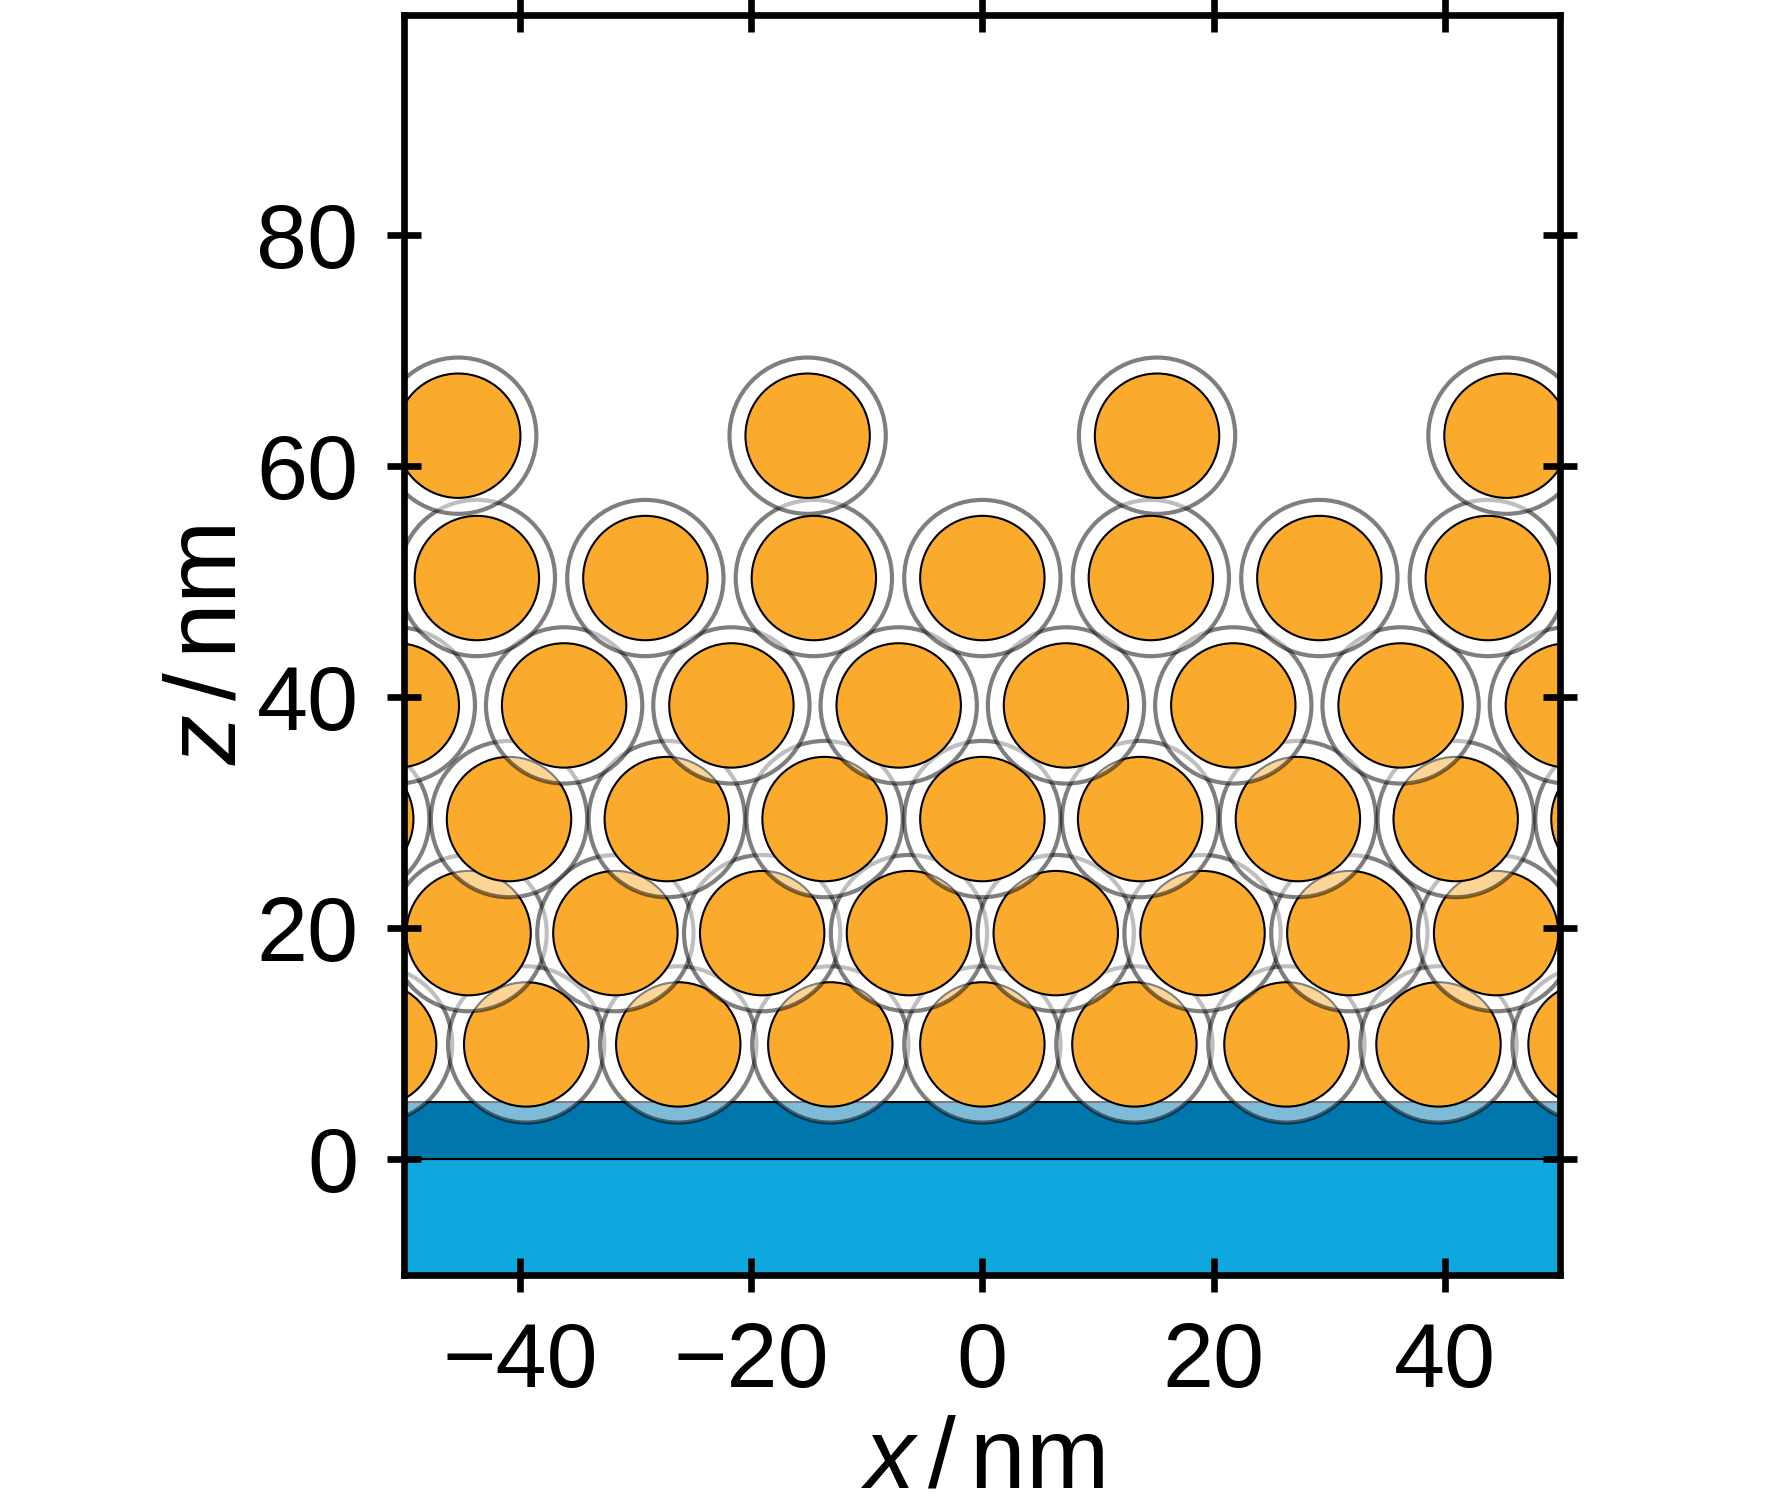
\includegraphics{looselyPackedNP_VerticalStructure_SC-IOS-11_PNRDepiction}
    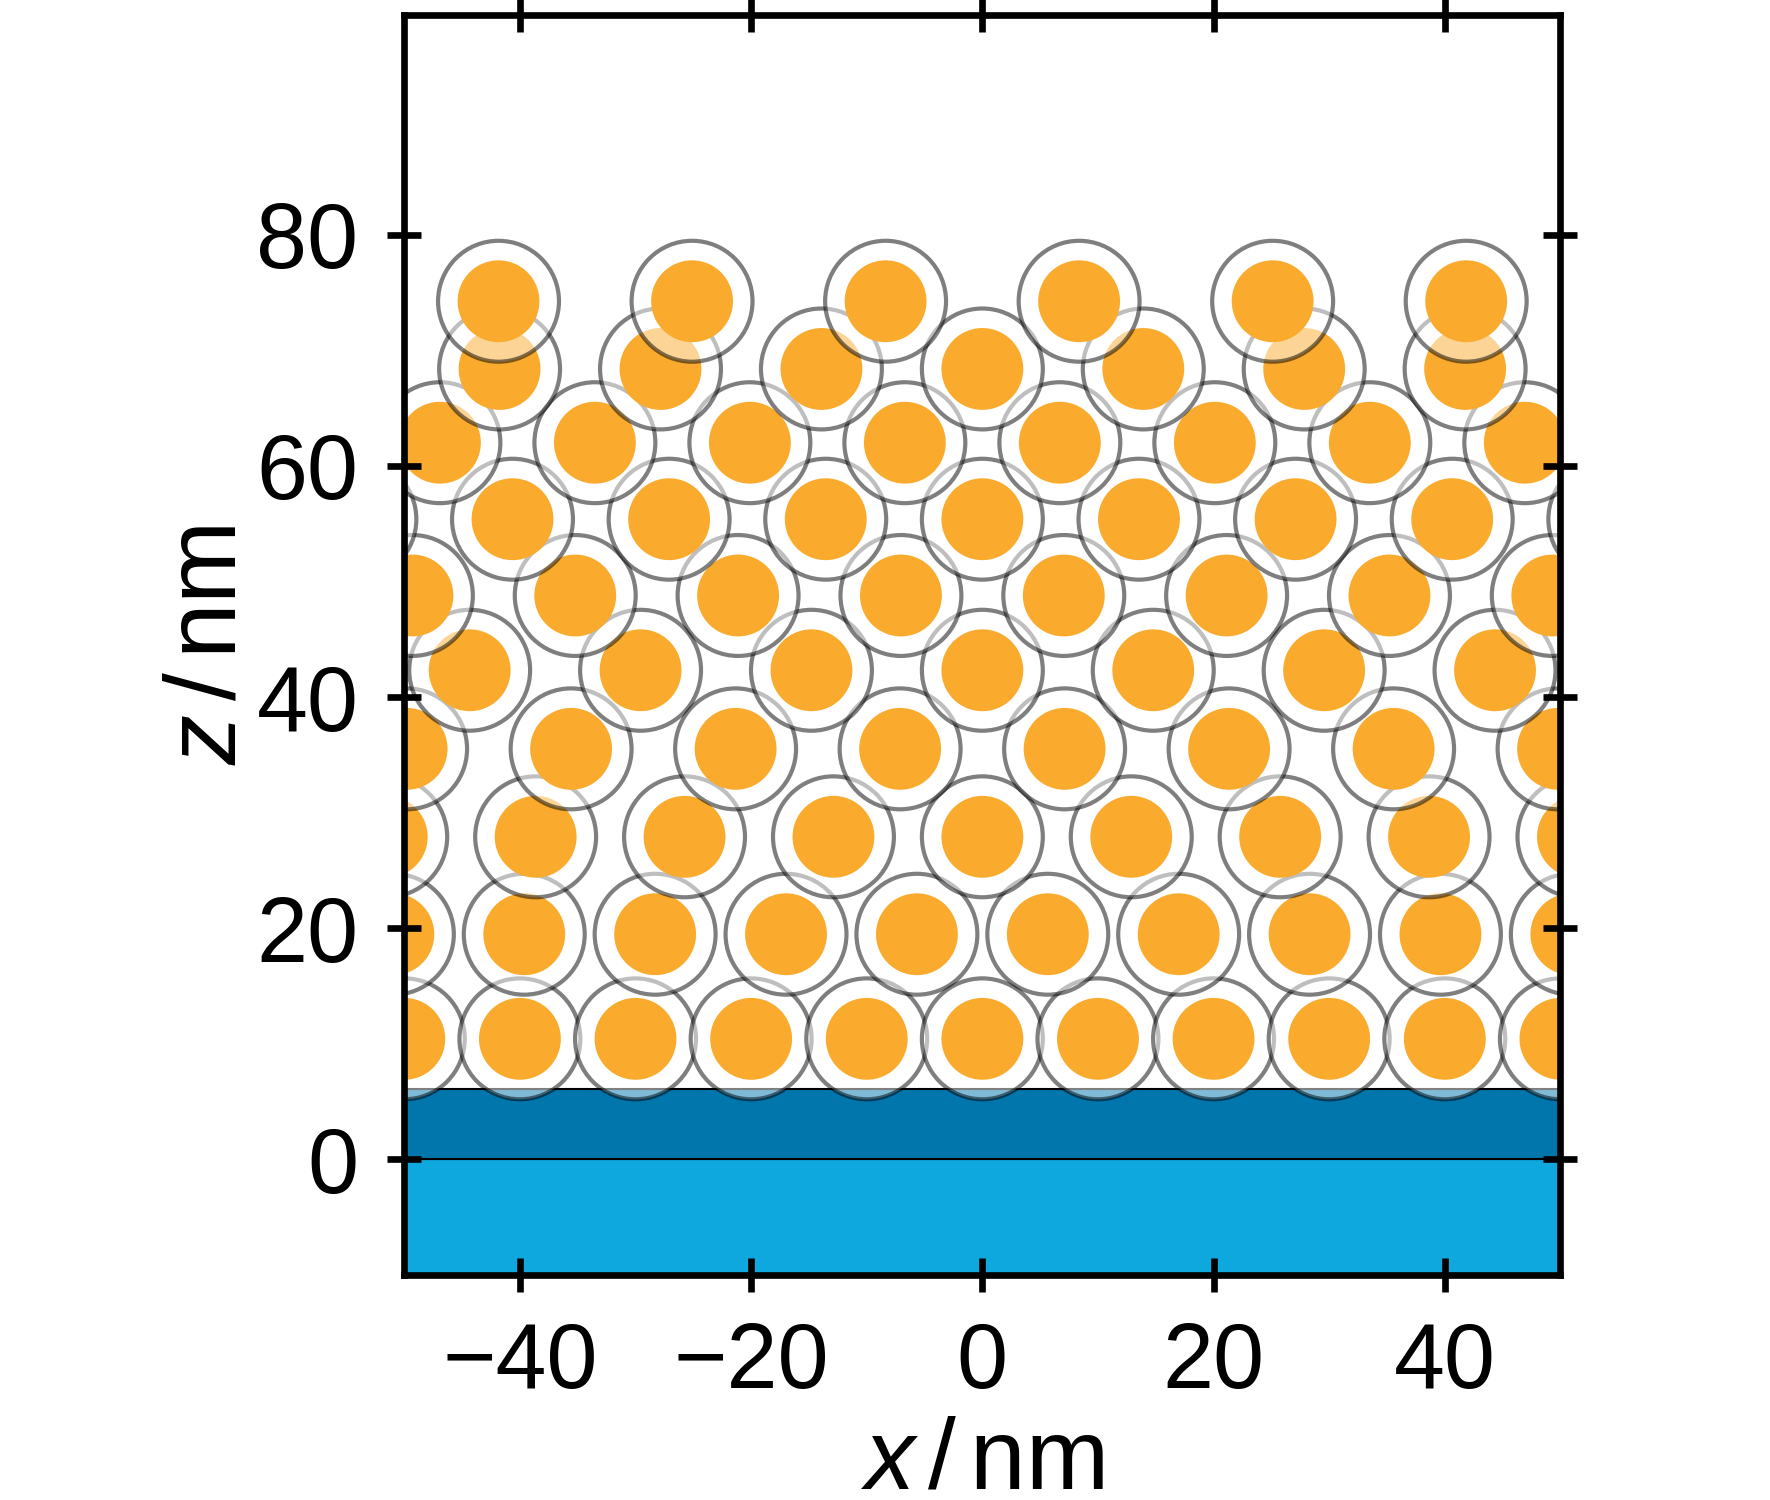
\includegraphics{looselyPackedNP_VerticalStructure_SC-IOS-7_PNRDepiction}
    \caption{\label{fig:looselyPackedNP:layer:pnrDepiction}Depiction generated from the fitted parameters in \reftab{tab:looselyPackedNP:nanoparticle:xrr} showing the average particle distance and layer packing.}
  \end{figure}

  \begin{figure}[tb]
    \centering
    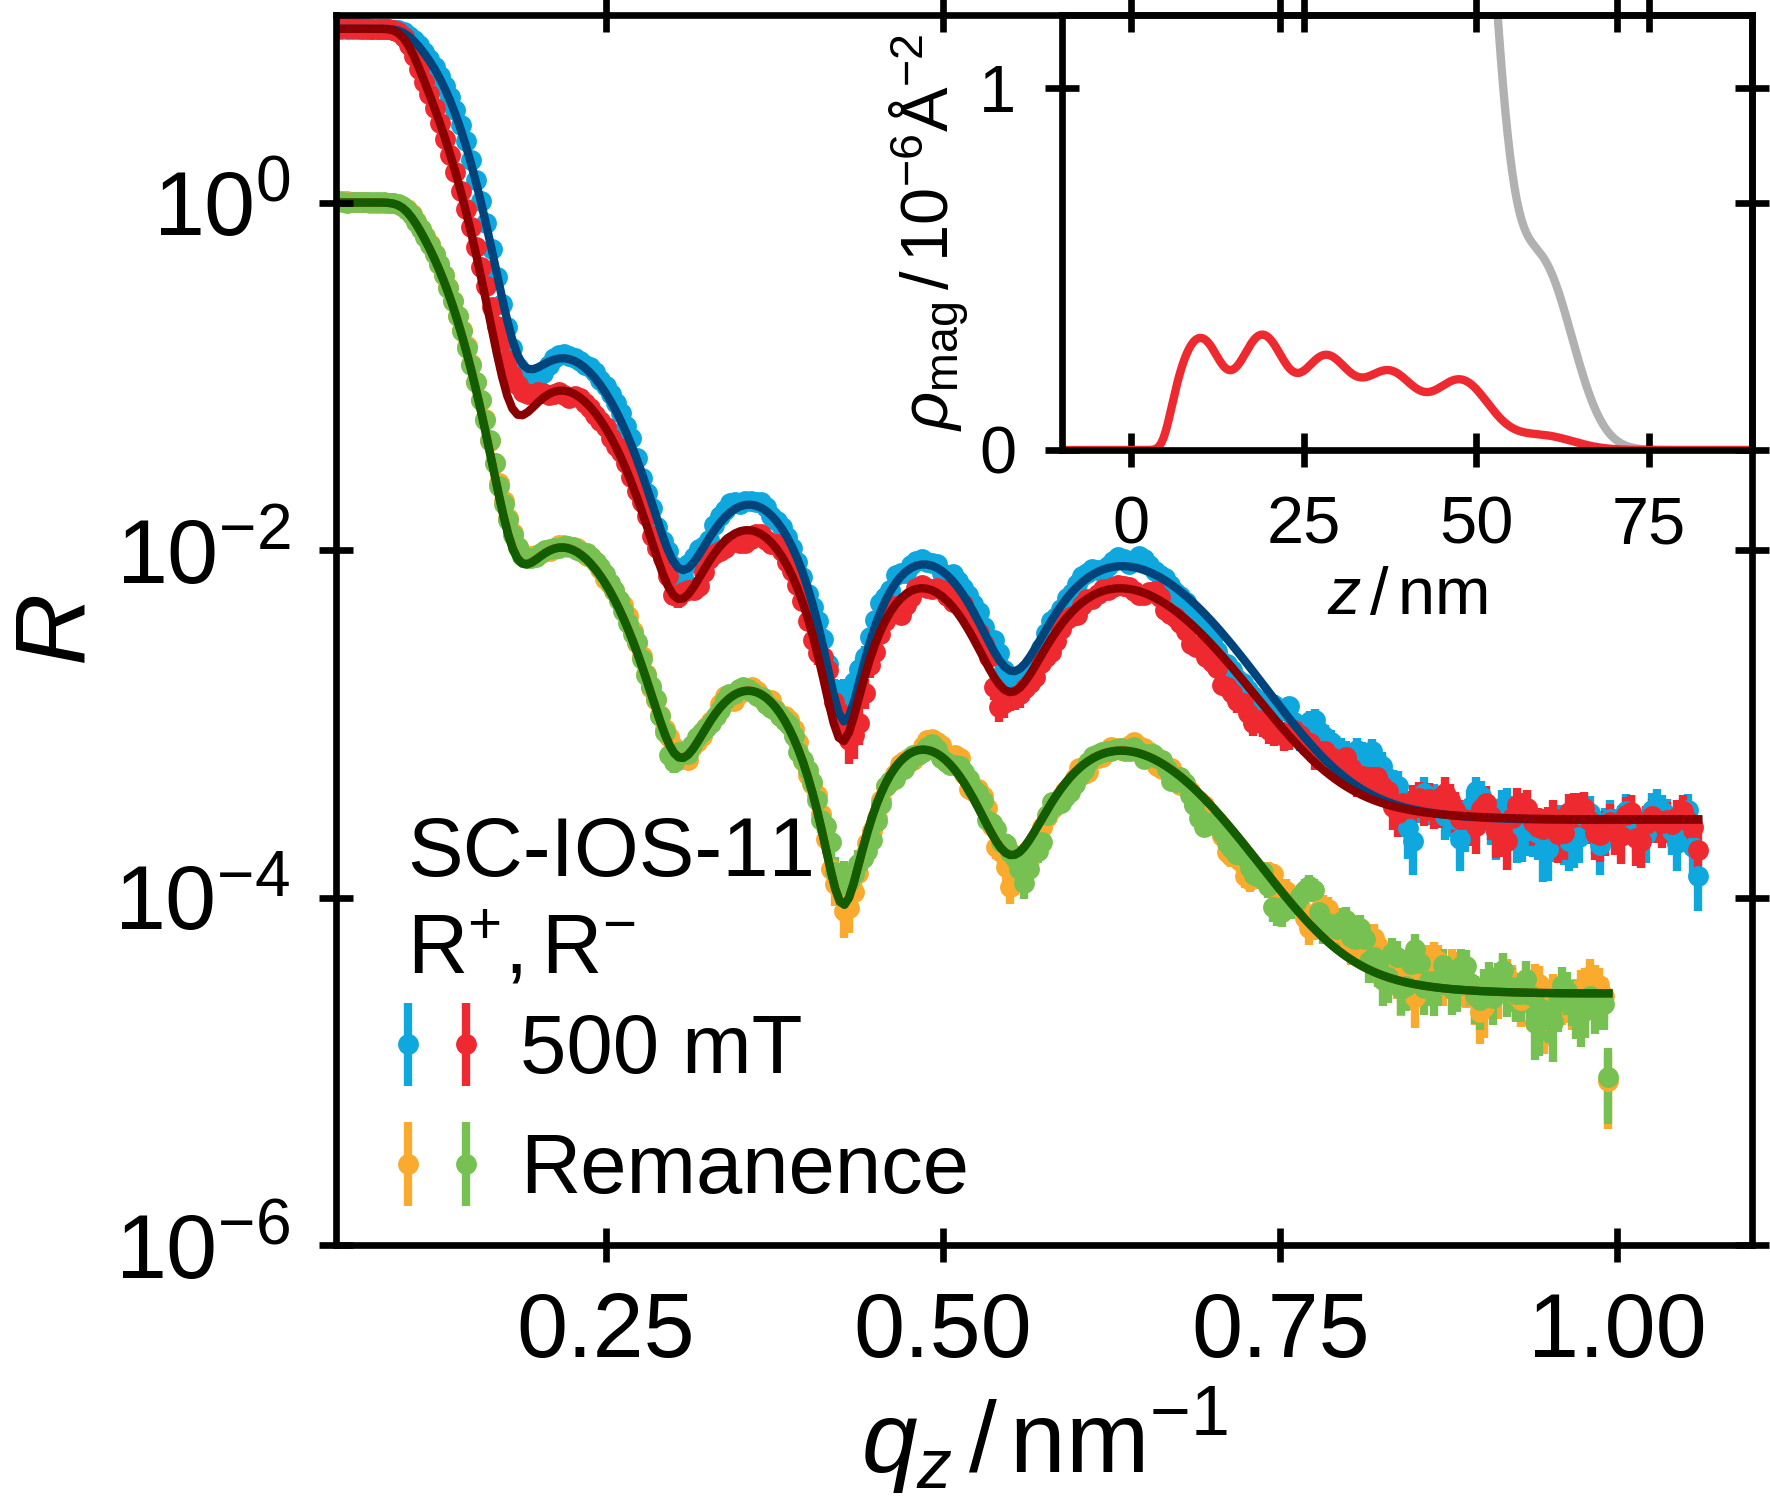
\includegraphics{looselyPackedNP_VerticalStructure_SC-IOS-11_PNR300K_500mT}
    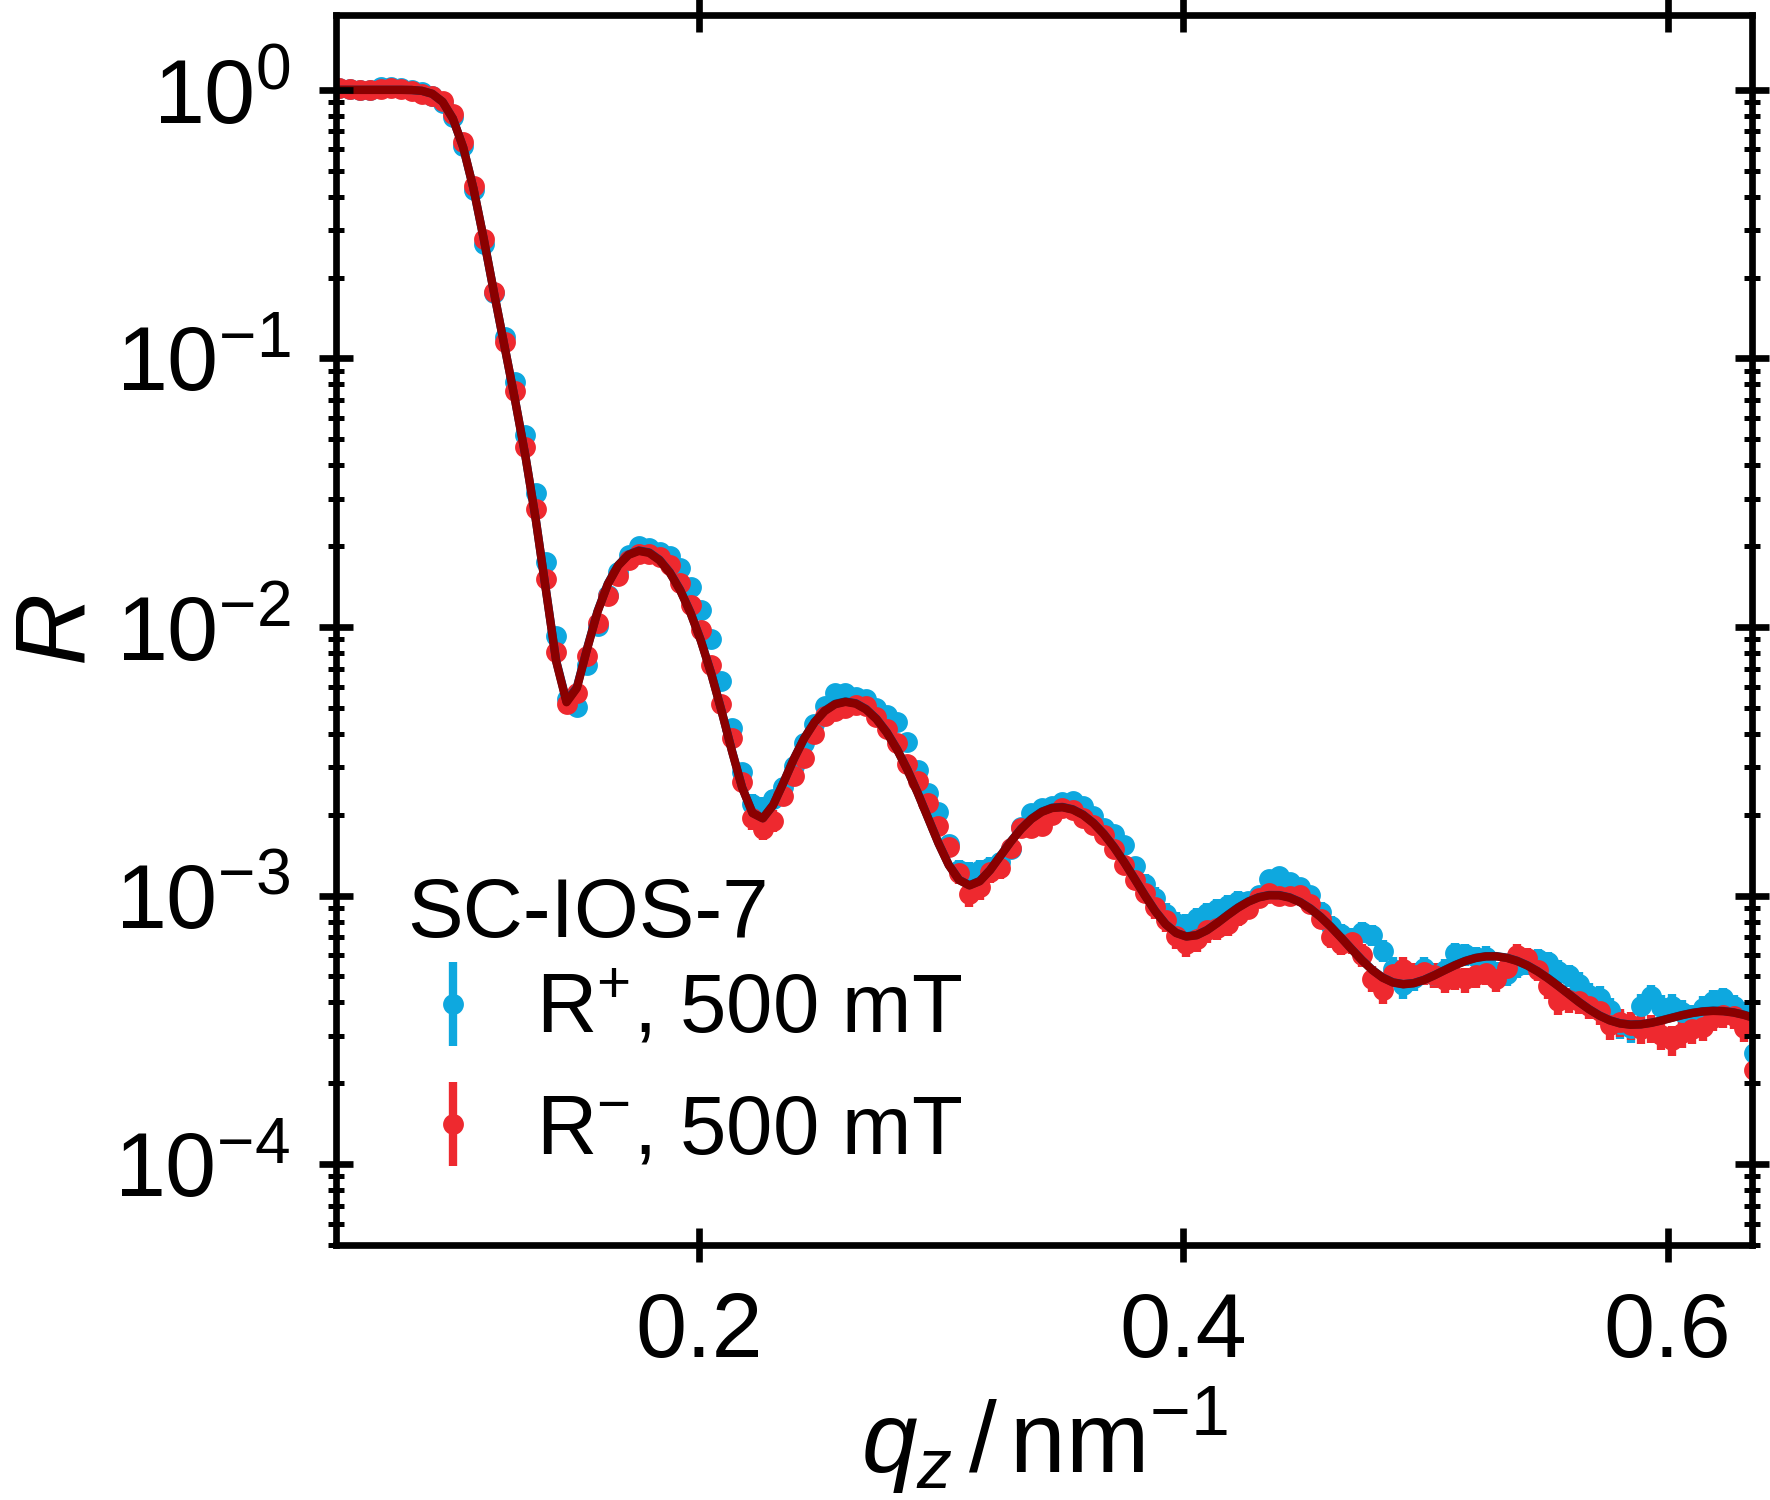
\includegraphics{looselyPackedNP_VerticalStructure_SC-IOS-7_PNR300K_500mT}
    \caption{\label{fig:looselyPackedNP:layer:pnrRoomTemperatureMagnetic}Room temperature polarized neutron reflectivity ($R^{+},\, R^{-}$) of SC-IOS-11 (left) and SC-IOS-7 (right). For SC-IOS-11 the PNR measured after removal of the field at remanence is additionally shown.}
  \end{figure}
  

  \begin{figure}[tb]
    \centering
    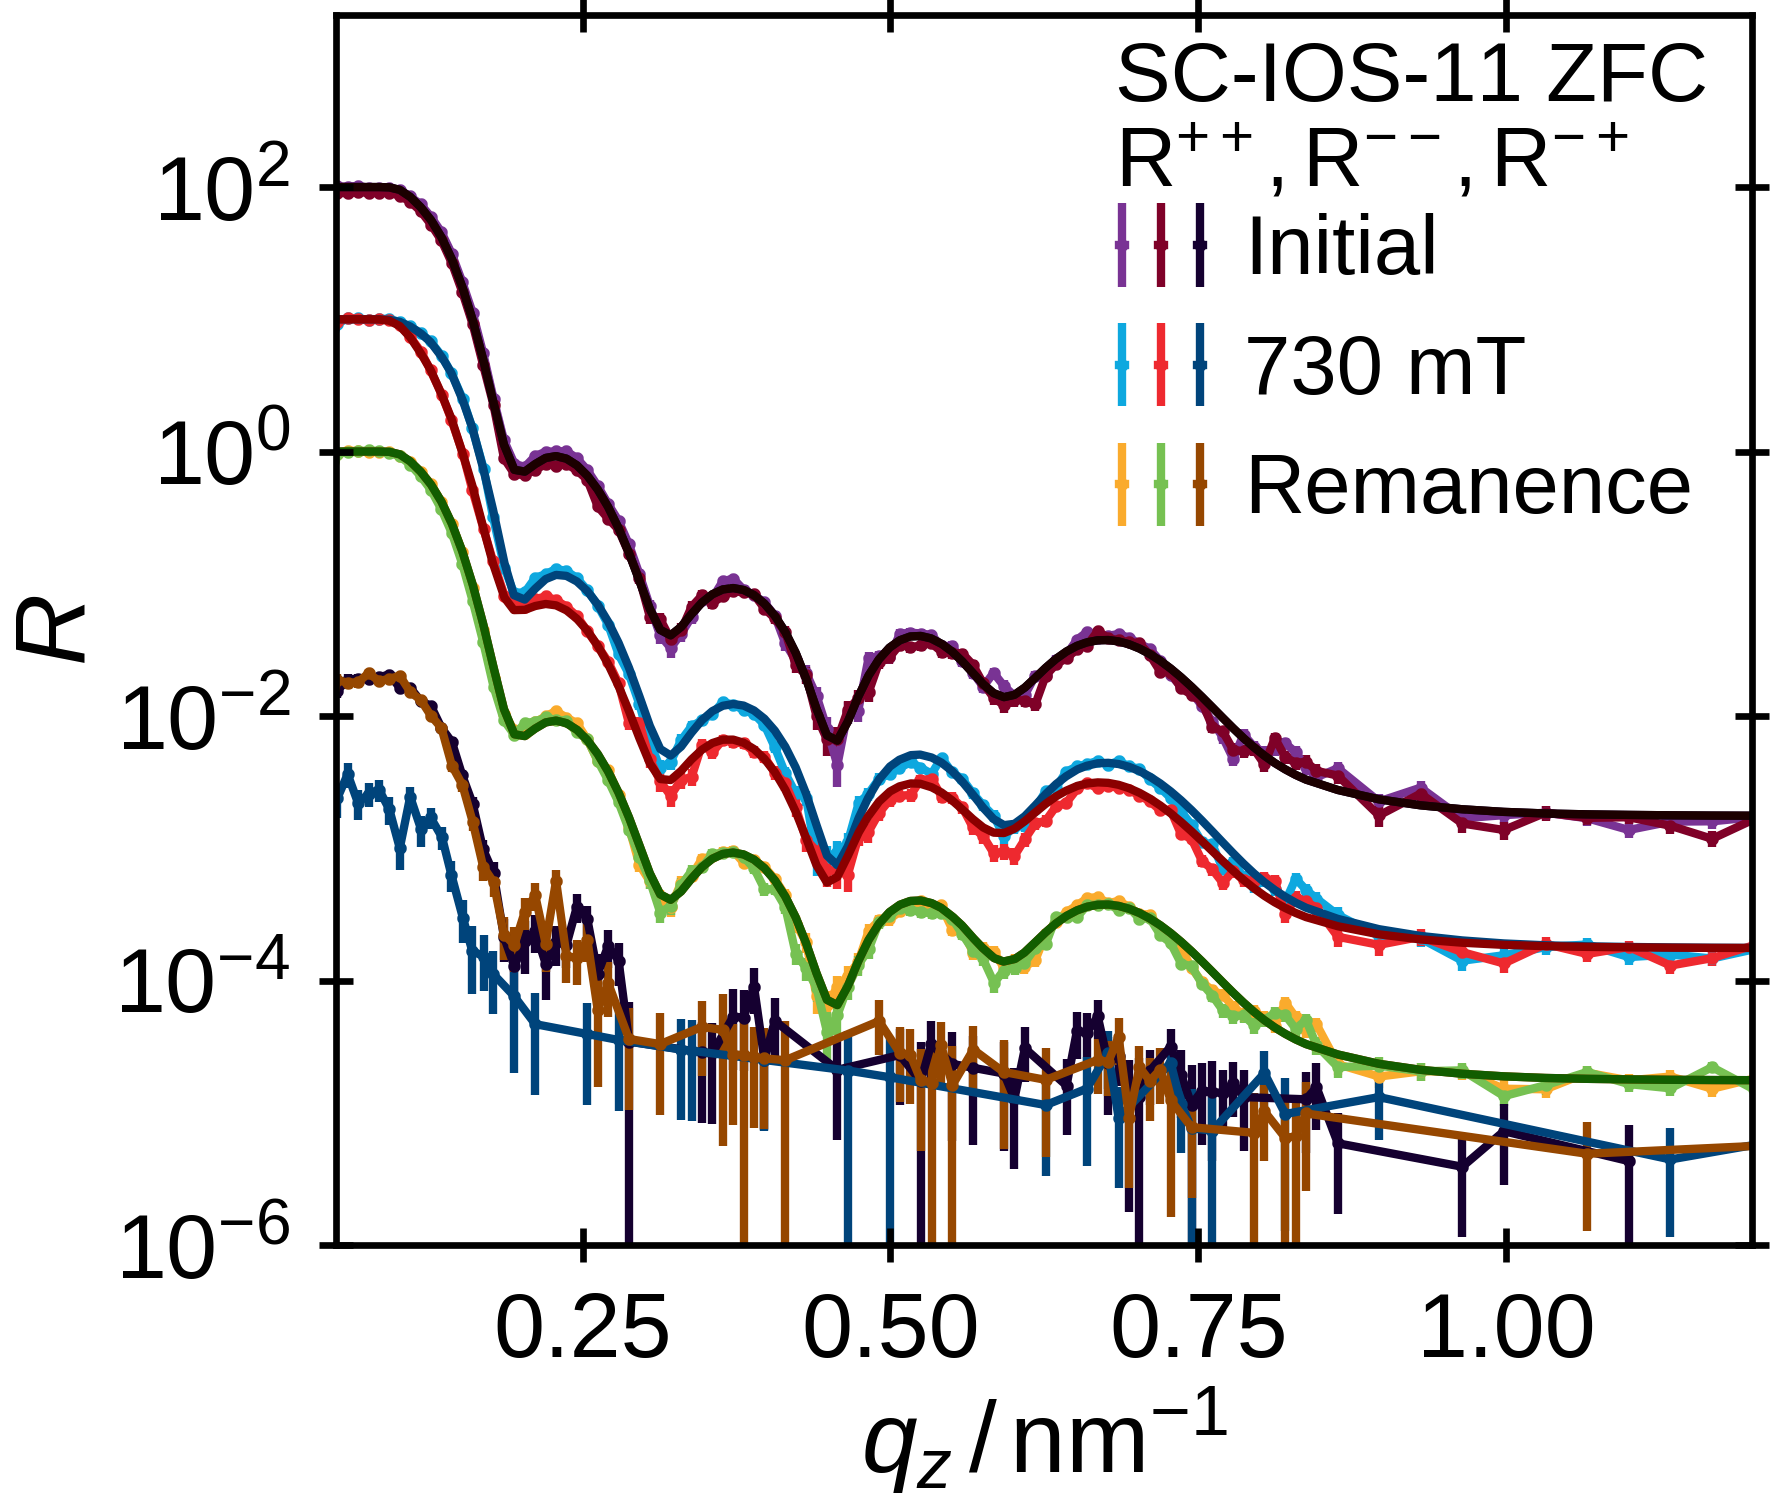
\includegraphics{looselyPackedNP_VerticalStructure_SC-IOS-11_PNR_ZFC30K}
    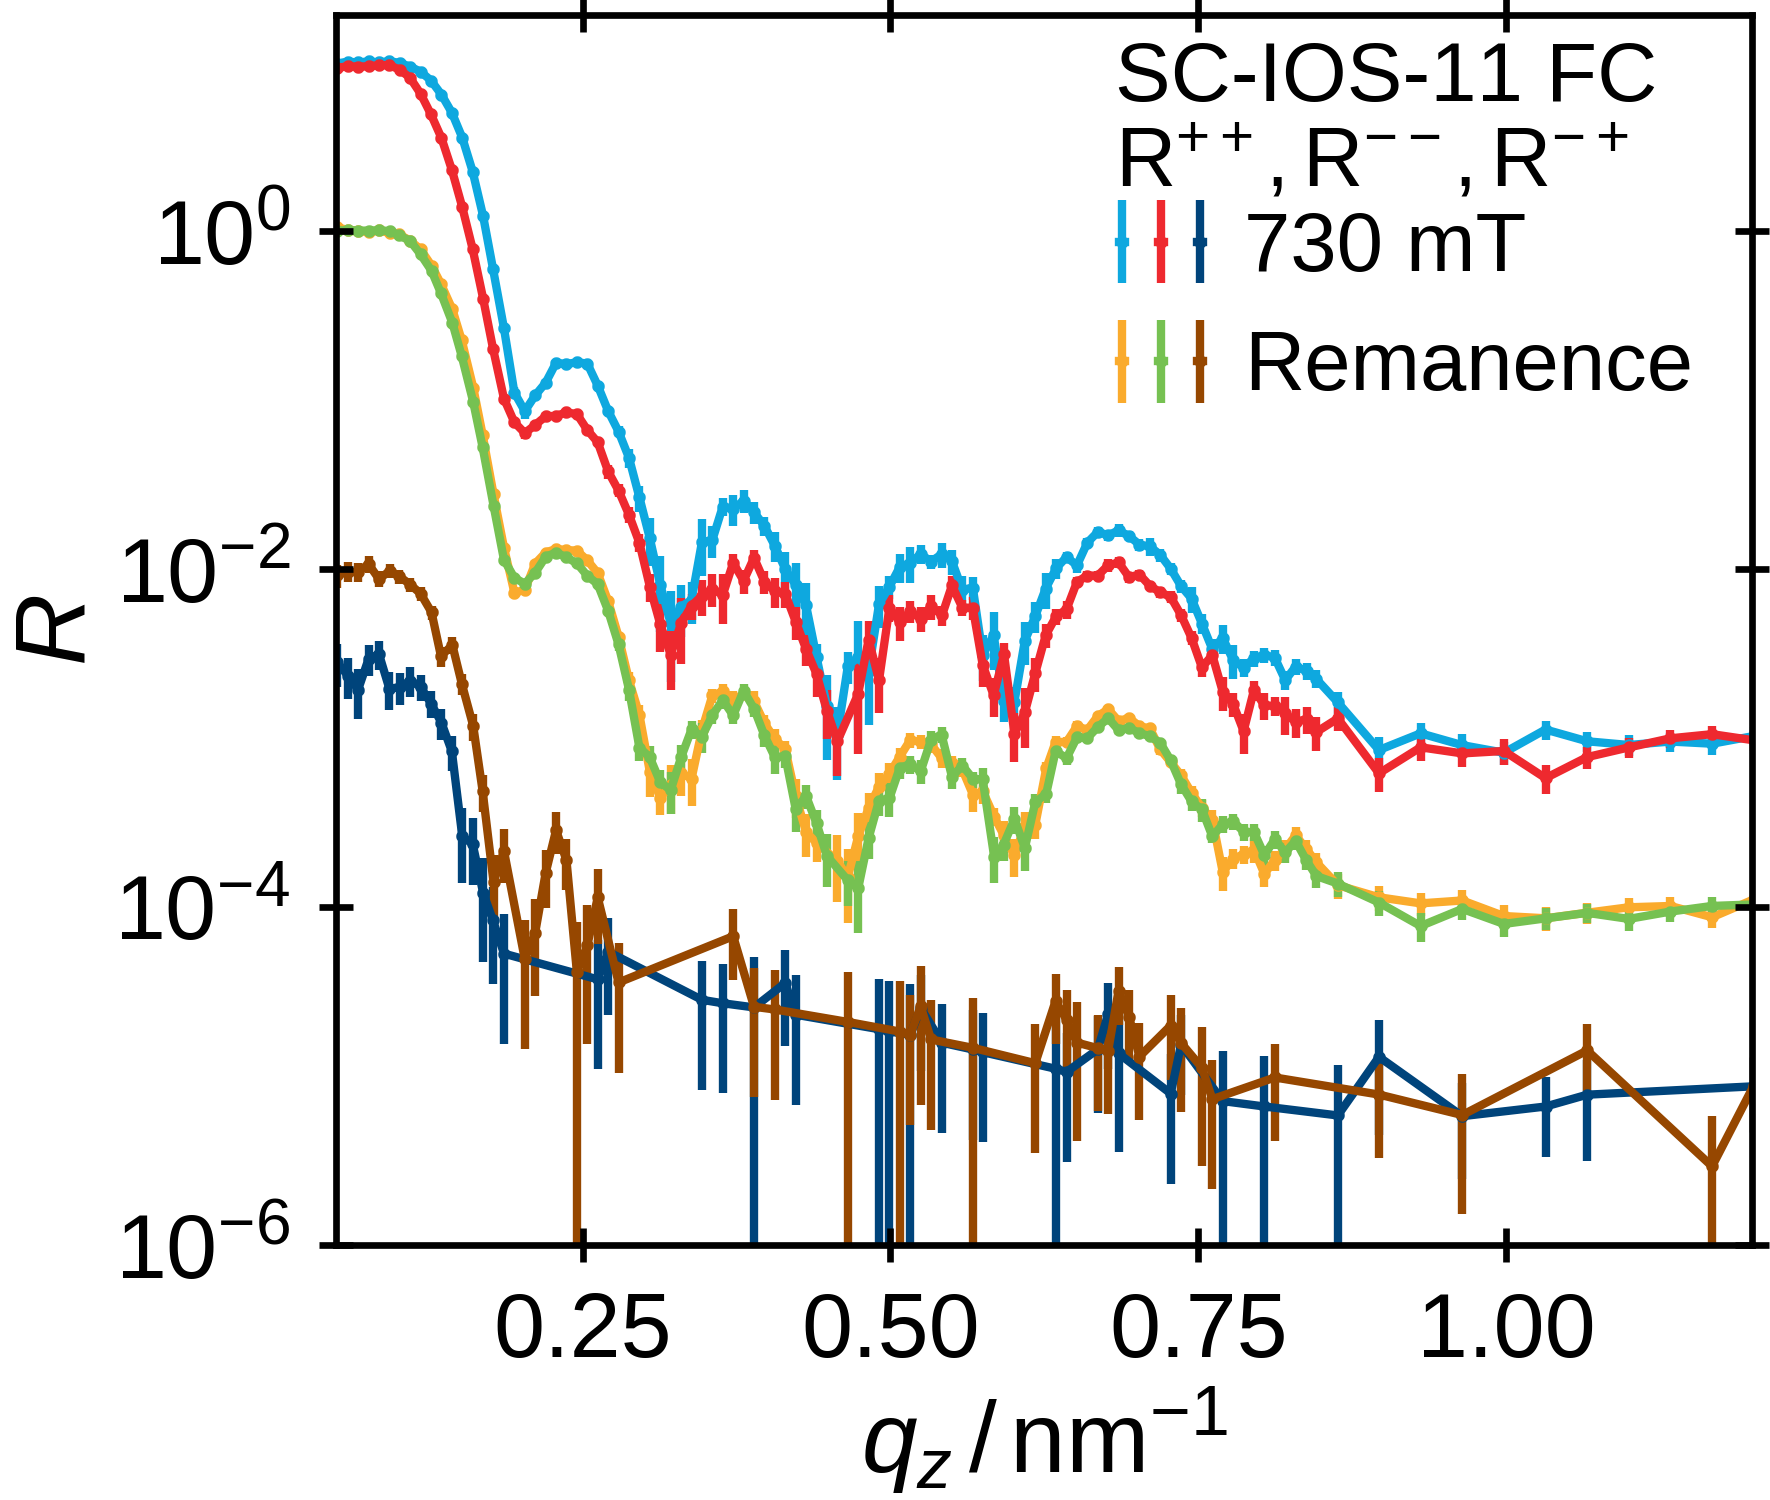
\includegraphics{looselyPackedNP_VerticalStructure_SC-IOS-11_PNR_FC30K}
    \caption{\label{fig:looselyPackedNP:layer:pnrZFCFCIOS11}Zero-field-cooled (left) and Field-cooled non-spin-flip reflectivity ($R^{++},\,R^{--}$) and spin-flip reflectivity ($R^{-+}$) of SC-IOS-11 at a magnetic field of $730 \unit{mT}$ and in remanence. For the zero-field cooled the initial reflectivity after cooling at guide field is additionally shown.}
  \end{figure}

  \begin{figure}[tb]
    \centering
    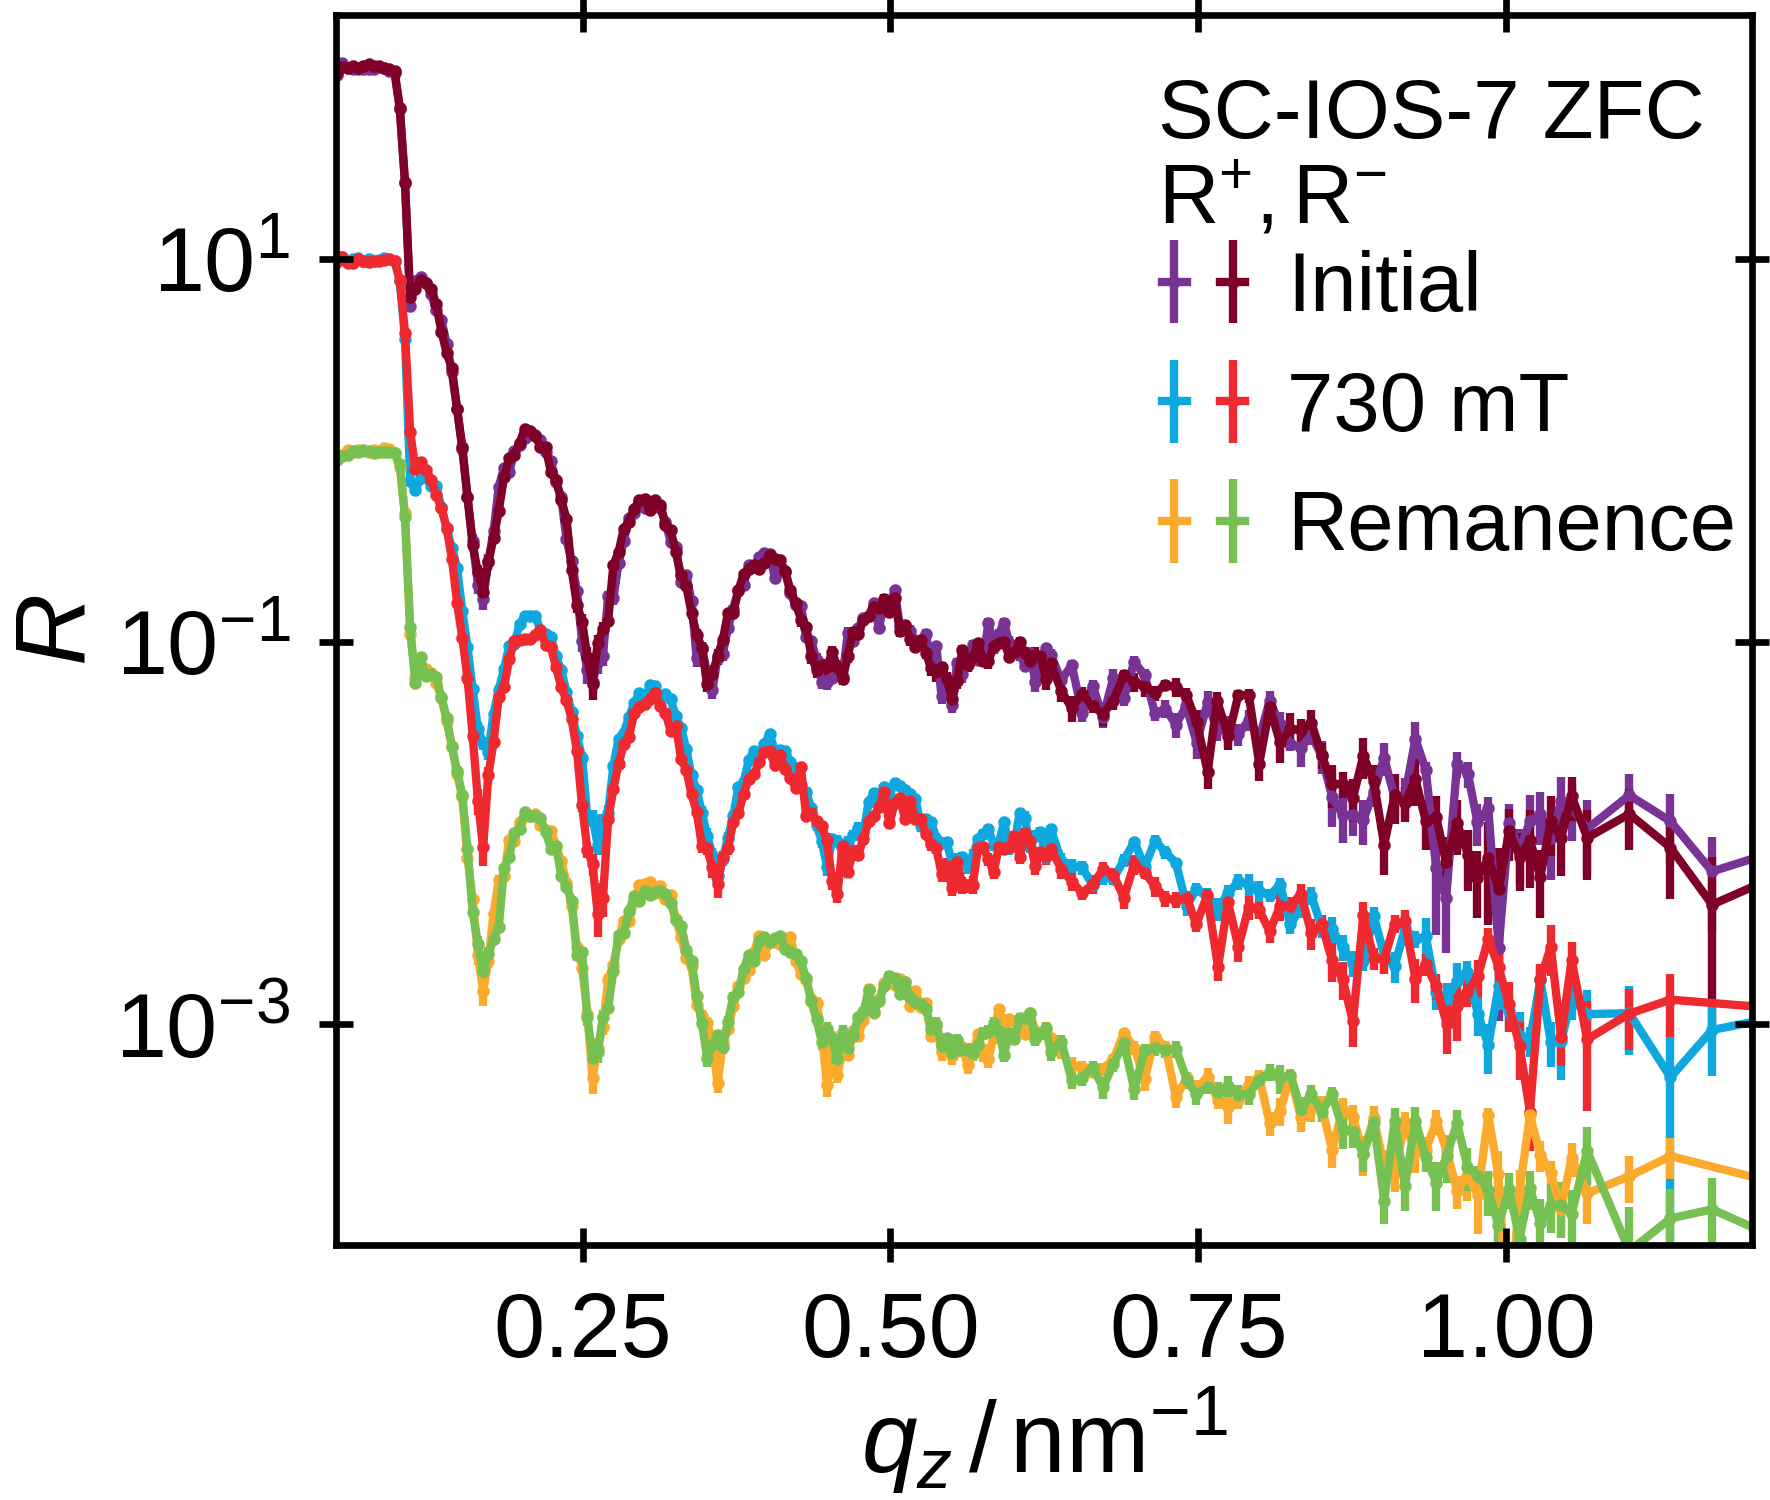
\includegraphics{looselyPackedNP_VerticalStructure_SC-IOS-7_PNR_ZFC30K}
    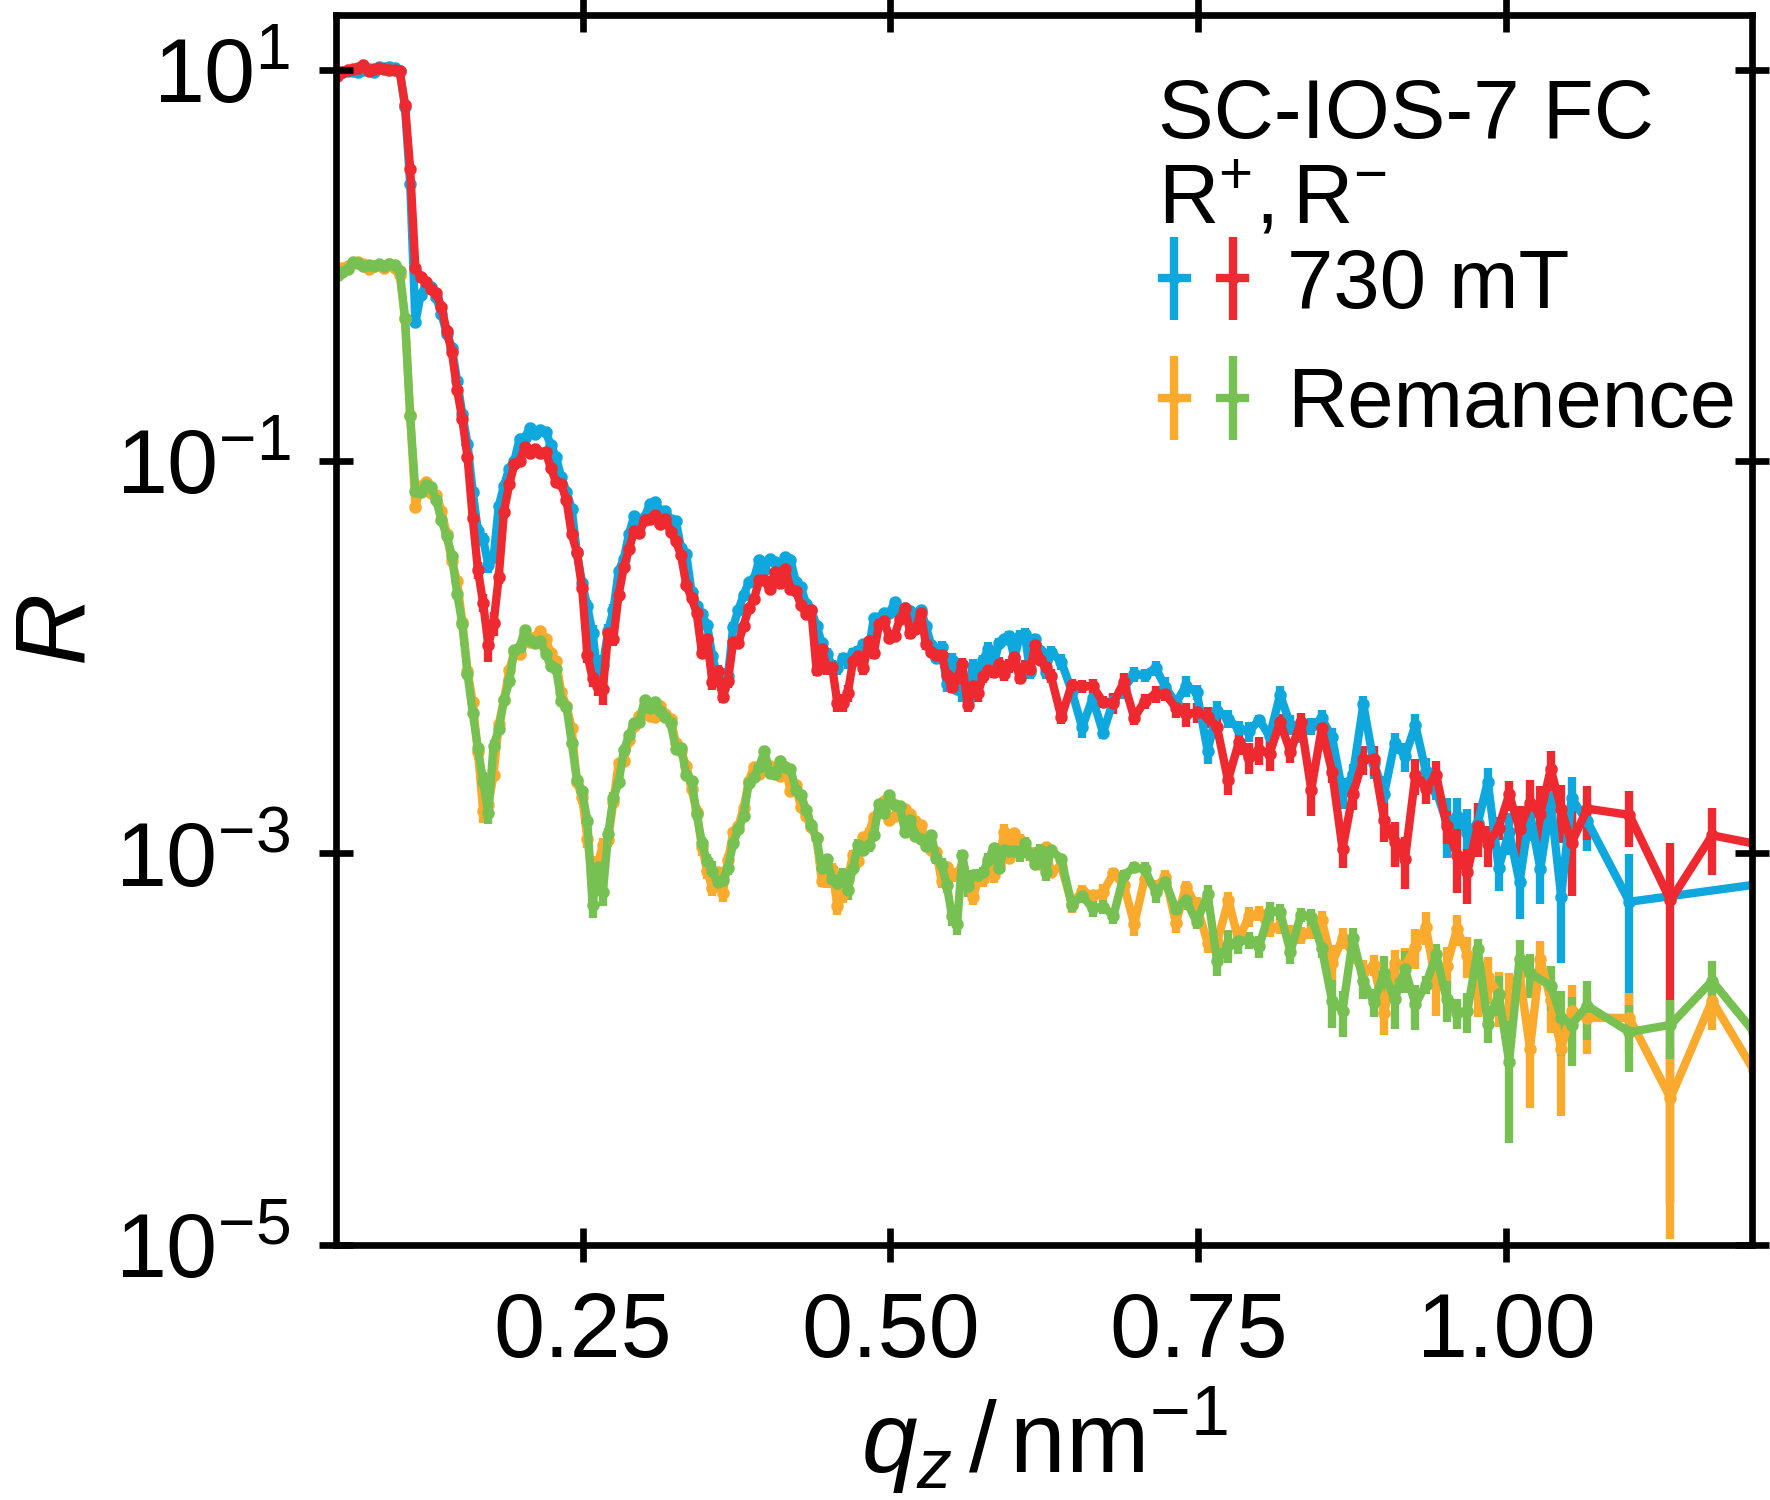
\includegraphics{looselyPackedNP_VerticalStructure_SC-IOS-7_PNR_FC30K}
    \caption{\label{fig:looselyPackedNP:layer:ZFCFCIOS7}Zero-field-cooled (left) and Field-cooled reflectivity of SC-IOS-7 at a magnetic field of $730 \unit{mT}$ and in remanence. For the zero-field cooled the initial reflectivity after cooling at guide field is additionally shown.}
  \end{figure}
\end{document}